\documentclass[tikz,border=3.14mm]{standalone}
\begin{document}
    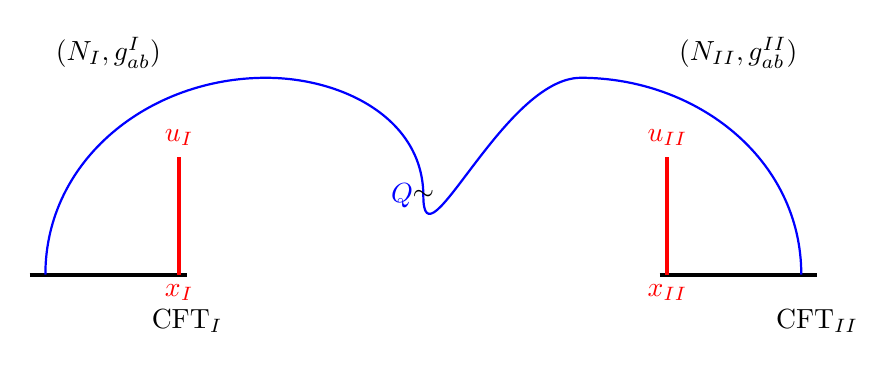
\begin{tikzpicture}
        % Draw the two black horizontal lines
        \draw[line width=0.5mm] (-5,0) -- (-3,0) node[align=center, below, yshift=-0.3cm]{CFT$_{\text{I}}$};
        \draw[line width=0.5mm] (3,0) -- (5,0) node[align=center, below, yshift=-0.3cm]{CFT$_{\text{II}}$};
        
        % Draw the two blue curves
        \draw[thick, blue] (-4.8,0) to[out=90,in=180] (-2,2.5) to[out=0,in=90] (0,1);
        \draw[thick, blue] (0,1) to[out=270,in=180] (2,2.5) to[out=0,in=90] (4.8,0);
        
        % Mark the interface brane Q
        \draw[thick] (0,1) node[blue, left]{$Q$} node{$\sim$}; % Adding wave-like symbol
        
        % Mark the points and red lines
        \draw[red, line width=0.5mm] (-3.1,0) -- (-3.1,1.5) node[red, above]{$u_{\text{I}}$};
        \draw[red, line width=0.5mm] (3.1,0) -- (3.1,1.5) node[red, above]{$u_{\text{II}}$};
        
        % Label the points
        \draw (-3.1,0) node[below, red]{$x_{\text{I}}$};
        \draw (3.1,0) node[below, red]{$x_{\text{II}}$};
        
        % Label the dual CFTs and their corresponding bulks
        \draw (-4,2.5) node[above]{$(N_{\text{I}},g^{\text{I}}_{ab})$};
        \draw (4,2.5) node[above]{$(N_{\text{II}},g^{\text{II}}_{ab})$};
    \end{tikzpicture}
\end{document}